
\section{Running}


There are 3 different ways to run the application. But first open up
Eclipse, which has been previously have set
up.

\subsection{Debugging inside of
Eclipse}\label{debugging-inside-of-eclipse}

\begin{enumerate}
\def\labelenumi{\arabic{enumi}.}
\item
  Create a \emph{Run Configuration} with ``jetty:run'' as goal for the
  \emph{webapp} project. See figure \ref{run01}.
  
\item
  Save configuration and run it. If the program runs properly the
  console should look something like in figure \ref{run02}.
\item
  Use your browser to open http://localhost:8080/election
\end{enumerate}

\begin{figure}[htbp]
\centering
  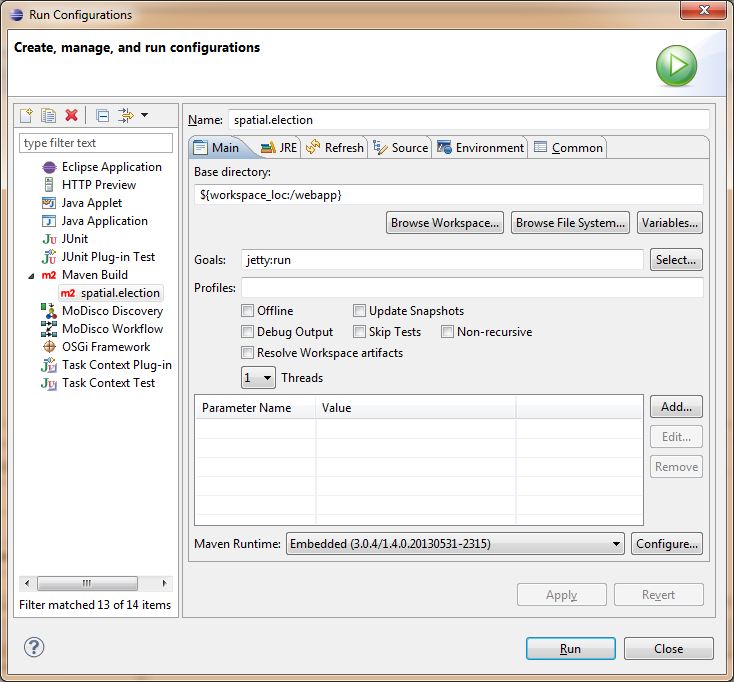
\includegraphics[width=1.1\textwidth]{../img/dwACYmd.png}
\caption{Eclipse run configuration}
\label{run01}
\end{figure}

\begin{figure}[htbp]
\centering
  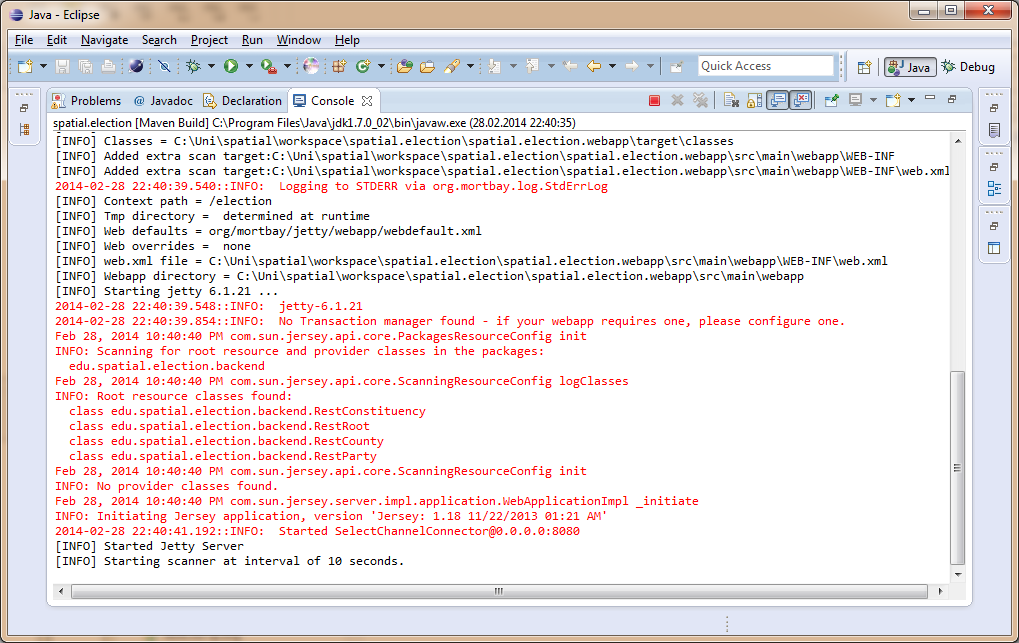
\includegraphics[width=1.1\textwidth]{../img/UZXVJIp.png}
\caption{Eclipse project run in Console view}
\label{run02}
\end{figure}

\begin{center}\rule{3in}{0.4pt}\end{center}

\subsection{Running a build executable
jar}\label{running-a-build-executable-jar}

\begin{enumerate}
\def\labelenumi{\arabic{enumi}.}
\itemsep1pt\parskip0pt\parsep0pt
\item
  Run the Maven command ``Install'' on the root project, to build all
  files. See figure \ref{run03}
  
\item
  The build might take some seconds. In the end there should be an
  ``BUILD SUCCESS''. See figure \ref{run04}
  
  
\item
  Go to the ``server'' subproject directory, navigate to target. There
  you should find an executable jar. You can start it with \emph{java
  -jar {[}\ldots{}{]}.jar}. The command window should look like in figure
  \ref{run05}.
  
  
  
\item
  Use your browser to open http://localhost:9191/
\end{enumerate}

\begin{figure}[htbp]
\centering
  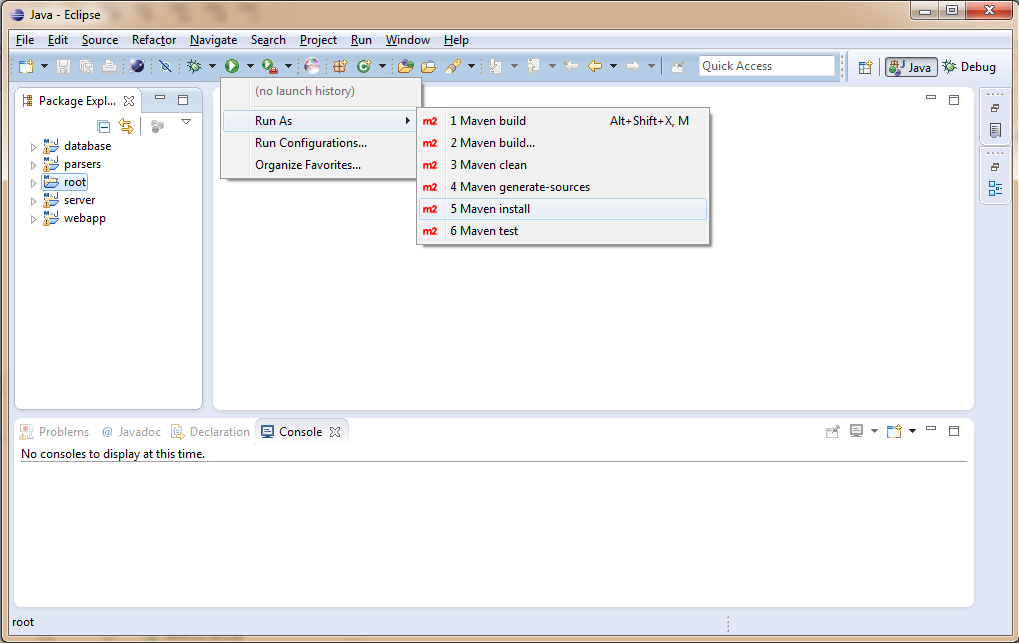
\includegraphics[width=1.1\textwidth]{../img/fvcN51B.png}
\caption{Eclipse Maven install run}
\label{run03}
\end{figure}


\begin{figure}[htbp]
\centering
  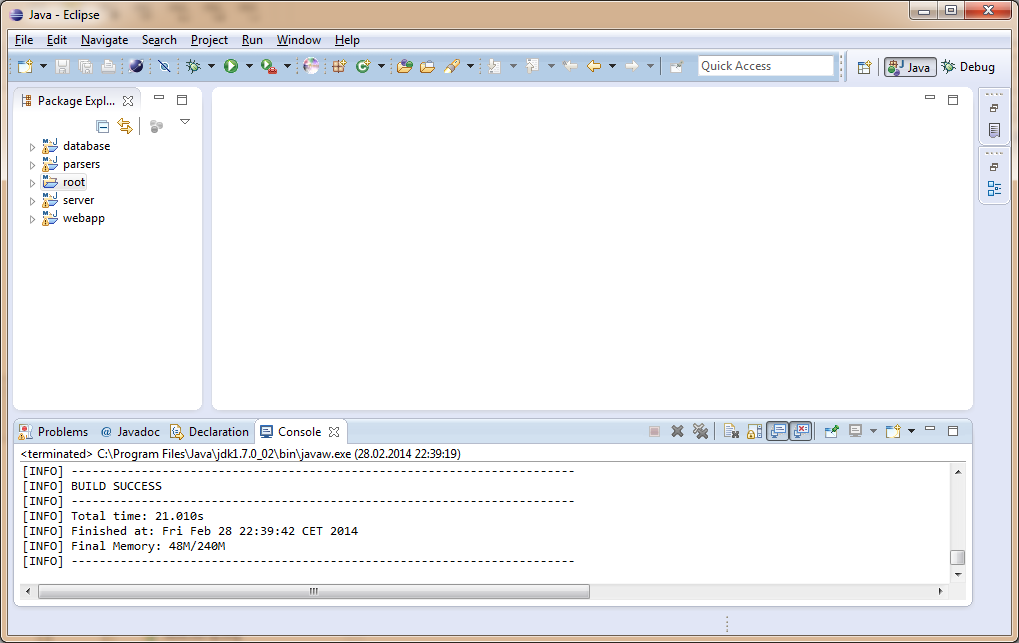
\includegraphics[width=1.1\textwidth]{../img/v13HHJO.png}
\caption{Eclipse Maven build successfuly}
\label{run04}
\end{figure}
  
  
\begin{figure}[htbp]
\centering
  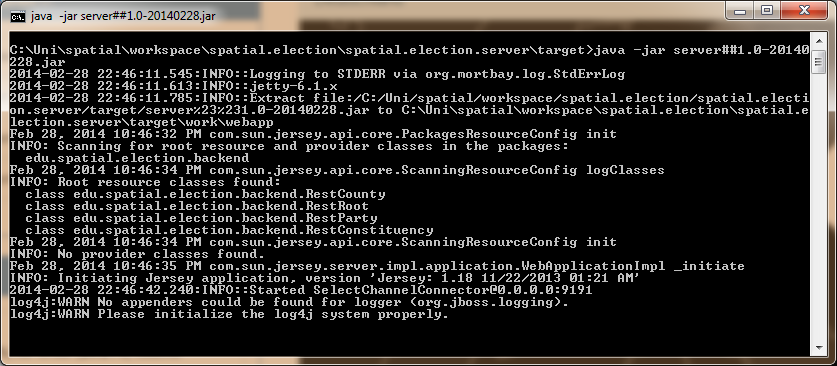
\includegraphics[width=1.1\textwidth]{../img/wFn3GVG.png}
\caption{Java execution of the project binary}
\label{run05}
\end{figure}

\begin{center}\rule{3in}{0.4pt}\end{center}


\subsection{Running a build war file with
Tomcat}\label{running-a-build-war-file-with-tomcat}

\begin{enumerate}
\def\labelenumi{\arabic{enumi}.}
\itemsep1pt\parskip0pt\parsep0pt
\item
  Follow the same steps from the previous part: Run the ``Install''
  command, wait for the ``BUILD SUCCESS'' message in the console.
\item
  Go to the ``server'' subproject directory, navigate to target. There
  you should find a war file. Import this file to your tomcat server.
  Usually its administration GUI is available from
  ``{[}\ldots{}{]}/manager/html/''.
\item
  After importing the war file, you should be able to click the link
  ``Spatial Election'' in the list of Tomcat applications. It will guide
  you to the project website.
\end{enumerate}